%\begin{itemize}
%    \item
%        Wie wird das mathematische Modell in Software implementiert?
%    \item
%        Wie wird die Kommunikation mit einem PC implementiert? (Protokoll)
%    \item
%        Event-System
%    \item
%        User-Interface am Ger\"at
%\end{itemize}


\subsubsection{Constraints for the uC programm}

The chosen  microcontroller dsPIC33ep  provides 16kB  of ROM  and 2kB  of RAM,
12bit resolution  in the ADC  and DAC and up  to 60 MIPS  computing power. The
anti-aliasing filter  of the  ADC is  set to  5khz, which  means that  we need
to  sample with  at  least  10khz. However the  LT3741  regulator takes  about
\SI{300}{\micro\second} to adjust  its output voltage --- 3  times longer then
our  sample rate. To  remedy  this  we use  Oversampling  by  factor 4,  which
has  the nice  benefits  of giving  us  an additional  bit  of resolution  and
making the anti-aliasing  filter simpler. The main routine  for the adjustment
of  the  regulator  should  not  use  more  than  25\%  of  the  CPU  time  and
must  run every  \SI{400}{\micro\second},  so  it must  not  take longer  than
\SI{100}{\micro\second} or about 6000 Instructions to finish one calculation.


\subsubsection{I-V Curve and Operating Points}
\label{subsec:iv-curve-operating-points}

The  I-V  curve  from  \eqref{eq:I-V} is implemented using a fixed point  library
supplied by Microchip. Since this library also provides an exponential function,
the implementation is made straightforward.

To  find the  target  operating point,  we calculate  the  load resistance  by
dividing  the actual  voltage  by  the actual  current  $R_{load}  = U_{is}  /
I_{is}$. Then we  draw the load line  $I = f(U) =  U / R_{load}$ and  find the
intersection with  the I-V curve  of the model.   This process is  pictured in
figure \ref{fig:model:approx}.   The intersection is  found by using  a binary
search algorithm,  which is  converging slower than  newton's method  but more
stable -- newton's method can fail if $V_T$ in \eqref{eq:I-V} is small.

If we want to use multiple curves to model the staircase characteristic shown in
figure \ref{fig:model:steps} we  need to determine which curve is applicable for
a given load. This process can be made less CPU intensive if we precalculate the
resistance-thresholds by finding the intersections between two curves.  There is
always exactly one intersection if  $V_{oc1} > V_{oc2}$ and $I_{sc1} < I_{sc2}$.

\begin{minipage}{0.5\textwidth}
	\center
    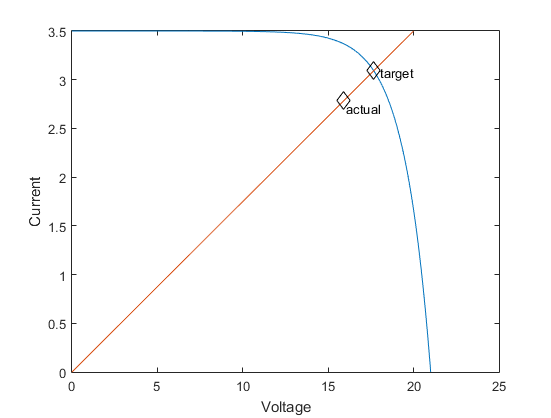
\includegraphics[width=.95\textwidth]{images/model/approx.png}
    \captionof{figure}{Actual and target operating points}
    \label{fig:model:approx}
\end{minipage}
\begin{minipage}{0.5\textwidth}
	\center
    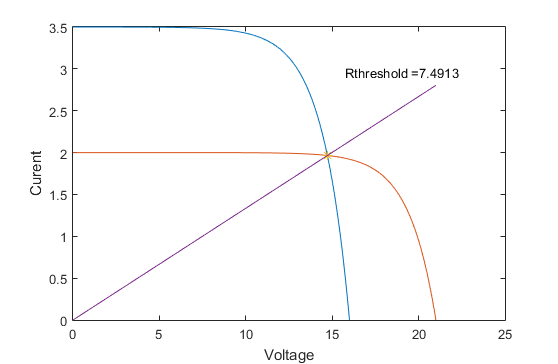
\includegraphics[width=.95\textwidth]{images/model/threshold.png}
    \captionof{figure}{Threshold resistance for selecting a curve}
    \label{fig:model:threshold}
\end{minipage}
